\newpage
\section{\texorpdfstring{\LaTeX{} 入门}{LaTeX入门}} 
\subsection{\texorpdfstring{\LaTeX{} 简介及与Word对比}{Latex简介及与Word对比}}

\subsubsection{\texorpdfstring{\LaTeX{} 简介}{LaTeX简介}}

%\newcommand{\XeLaTeX}{X\kern-.15em\lower.5ex\hbox{\sffamily\small e}\kern-.05em\LaTeX}
\LaTeX{}是一个基于\TeX{}的排版系统,最初由Leslie Lamport于1984年开发。
它是一个开源的文档排版系统,广泛用于学术界和科研领域,尤其在数学、物理、计算机科学等领域中被广泛使用。
与传统的文字处理软件(如Word)相比,\LaTeX{}具有更强大的排版能力和灵活性,
特别是在处理复杂的数学公式、图表和参考文献时,有非常好的表现。

中文编写主要用\XeLaTeX{}编译器,
它是\LaTeX{}的一个扩展,支持Unicode字符集,可以更好地处理中文字符。
文档类型可选择“ctexart”,意为使用了“ctex”宏包的“article”文档类型。
我们不作过多介绍,够用即可。

\subsubsection{与Word对比}

\LaTeX{}与Word的所见即所得不同,写\LaTeX{}文件更像是在写代码,
实际上就是编写程序,告诉编译器如何排版,而在写作内容时,完全不需要考虑排版。

我看到过一个比喻:用Word就像是开小汽车,开得好不好、稳不稳,全凭驾驶员的技术;
而使用\LaTeX{}就像是开火车,一旦铺好了铁轨,车就会按照轨道稳定行驶,
但是,要铺好这个轨道需要较深厚的\LaTeX{}功底,我们一般都是使用别人铺好的轨道(即模板)。
我这里\textbf{只围绕我的模板进行介绍,讲解如何使用我的模板},更高级的技巧有兴趣可自行学习。

学习\LaTeX{}是个长期的过程,但一旦学习到一定程度,就会发现它相对于Word又快又好。
下面是一个\LaTeX{}和Word学习曲线图:
\begin{figure}[!h]
    \centering
    \captionsetup{font={small, bf}, margin=60pt}
    \begin{tikzpicture}[
        >=stealth,clip=true,scale=0.75
    ]
        \draw[->, thick] (0,0) -- (6.5,0) node[right] {\small 学习成本};
        \draw[->, thick] (0,0) -- (0,6.7) node[left, rotate=270, xshift=2.7cm, yshift=-0.4cm] {\small 熟练程度/效率};
    
        \draw[blue, thick, domain=0:6.5] 
            plot(\x, {(exp(0.4*\x) -1)*0.5}) node[right] {\LaTeX};
        \draw[red, thick, domain=0:6.5] 
            plot(\x, {(ln(\x +1))*2}) node[right] {Word};
    
        \draw[fill=white] (1.5,5) rectangle (5.2,6.2);
        \draw[blue,thick] (1.7,5.8) -- (2.3,5.8) node[right,black] {\small\LaTeX 曲线};
        \draw[red,thick] (1.7,5.3) -- (2.3,5.3) node[right,black] {\small Word曲线};
    
    \end{tikzpicture} 
    \caption{学习曲线对比图} 
\end{figure} 

\newpage

\subsection{下载安装及使用}
与其它语言相同,想要在自己电脑上编译、运行,就需要搭建运行环境。
我个人推荐使用VS Code代码编辑器,功能强大。

具体如何安装、配置,请参考\textbf{\textcolor{blue}{\href{https://zhuanlan.zhihu.com/p/38178015}{知乎文章(点击即可进入)}}}。

\textbf{注意,}一定要逐步按照文章内容,进行到最后一步。

另外VS Code界面支持中文,可以自己寻找教程修改。

正确安装并配置环境后,在VS Code左上角点击“文件”,选择“打开文件夹”,
这个文件夹就是工作文件夹了,所有编辑及编译的文件都在这个文件夹中。
你们可以选择我这个“演示”打开查看。

里面的文件就可以作为模板,把里面的文件拷贝到自己的工作文件夹,
在此基础上修改,就可直接应用模板的各种样式。

以我这个演示文件夹为例,其结构如下:
\begin{center}
\begin{minipage}{0.8\textwidth}
\dirtree{%
.1 演示/.
    .2 content/.
        .3 chapter1.tex.
        .3 \dots .
    .2 image/.
    .2 main.tex.
    .2 content.tex.
    .2 informatin.tex.
    .2 abstract.tex.
    .2 titlepage.tex.
    .2 apendendices.tex.
    .2 references.bib.
    .2 \dots .
}
\end{minipage}
\end{center}

理论上来说,\LaTeX{}文档一个文件足矣,我这样拆开是秉持着“样式与内容分离”的理念。

文档主要信息,如作者等在information.tex中编辑,摘要在abstract.tex中编辑。
附录我们用不到,我给它关掉了,需要用的话在主文件main.tex中打开(一般情况下不用打开main.tex),再编辑appendices.tex即可。

编写文档时,只需编辑content文件夹中的章节文件,然后再content.tex中添加所需文件即可。

参考文献以references.bib形式储存。图片储存在image文件夹中,其它文件就是辅助文件了。

main.pdf就是输出的文档。

\subsection{基础命令}
\subsubsection{章节与段落}

如果你只是编辑一些文字内容,可以直接在content文件夹中新建章节文件,
然后在content.tex中添加进去。

比如新建了一个chapter1.tex文件,在其中写入:
\begin{center}
\begin{minipage}{0.8\textwidth}
    \hspace{1em}
\begin{lstlisting}[language={[LaTeX]TeX}]
    \section{文献管理软件}
    \subsection{介绍}
    
    写论文最好有一个文献管理软件,方便管理参考文献。常用的有 EndNote、Mendeley、Zotero 等。
    我们学校已经购买了 Endnote 正版授权,可以到\textbf{\textcolor{blue}{\href{https://zbhrj1.jlu.edu.cn/download/EndNote21W.html}{吉大正版网站}}}下载使用。
    但是界面是全英文的,使用操作也不符合我的习惯,我这里只介绍我在用的Zotero,使用应该大同小异。
    
    
    
    \subsection{下载安装}
    
    Zotero基础功能免费,高级功能(如大容量云盘同步)是需要付费的,不过我们基本只用得到免费功能。
    软件可以在\textbf{\textcolor{blue}{\href{https://www.zotero.org/}{Zotero官方网站}}}直接下载使用。
\end{lstlisting}
\end{minipage}
\end{center}

\backslash section就是节标题,
同理\backslash subsection、\backslash subsubsection就是二三级节标题。
代码内换行编译出来是不换行的,换行在代码里体现是空一行,或者命令\backslash par。效果见本文档的效果见本文档开头(这就是本文档的代码)。
\\另外还有强制换行命令两个反斜杠\backslash\backslash ,但它只是换行,没有开启新的段落,这句话就是用了两个反斜杠换行的。

代码中的空格也不会参与编译,需要用到空格命令,这里介绍三种:

\begin{center}
\begin{minipage}{0.8\textwidth}
    \hspace{1em}
\begin{lstlisting}[language={[LaTeX]TeX}]
    a\qquad b % 两个字符空格

    a\quad b  % 一个字符空格 
    
    a\ b      % 小空格
\end{lstlisting}
\end{minipage}
\end{center}

效果如下:
\begin{center}
\begin{minipage}{0.8\textwidth}
a\qquad b 

a\quad b 

a\ b 
\end{minipage}
\end{center}

可以使用换页命令换页:
\begin{center}
\begin{minipage}{0.8\textwidth}
    \hspace{1em}
\begin{lstlisting}[language={[LaTeX]TeX}]
\newpage
\end{lstlisting}
\end{minipage}
\end{center}

\subsubsection{数学环境}

\LaTeX{}可以方便地输入美观的公式,下面介绍三种:

\begin{center}
\begin{minipage}{0.8\textwidth}
    \hspace{1em}
    \begin{lstlisting}[language={[LaTeX]TeX}]
        % 行内公式
        牛顿第二定律表述为:$F=ma$;
        % 单行不编号公式
        \[
            \int_{-1}^{1}x^2 \textrm{d}x=\frac{2}{3};
        \]
        % 单行编号公式
        \begin{equation}
            \int_{-1}^{1}x^2 \textrm{d}x=\frac{2}{3};
        \end{equation}
        % 多行编号公式
        \begin{align}
            \int_{-1}^{1}x^2 \textrm{d}x&=\left[\frac{1}{3}x^3\right]_{-1}^1\\
            &=\frac{2}{3}.
        \end{align}
\end{lstlisting}
\end{minipage}
\end{center}

效果如下:

牛顿第二定律表述为:$F=ma$;

\[
    \int_{-1}^{1}x^2 \textrm{d}x=\frac{2}{3};
\]

\begin{equation}
    \int_{-1}^{1}x^2 \textrm{d}x=\frac{2}{3};
\end{equation}

\begin{align}
    \int_{-1}^{1}x^2 \textrm{d}x&=\left[\frac{1}{3}x^3\right]_{-1}^1\\
    &=\frac{2}{3}.
\end{align}

如果要用无编号的equation或align,可替换成equation*或align*;
如果想要多行公式共用一个编号,可在equation中嵌套aligned。

\begin{center}
\begin{minipage}{0.8\textwidth}
    \hspace{1em}
\begin{lstlisting}[language={[LaTeX]TeX}]
        % 单行不编号公式
        \begin{equation}
            \int_{-1}^{1}x^2 \textrm{d}x=\frac{2}{3};
        \end{equation}
        % 多行单个编号公式
        \begin{equation}
            \begin{aligned}
                    \int_{-1}^{1}x^2 \textrm{d}x&=\left[\frac{1}{3}x^3\right]_{-1}^1\\
                    &=\frac{2}{3}
            \end{aligned}
        \end{equation}
\end{lstlisting}
\end{minipage}
\end{center}
    
效果如下:
\begin{equation*}
    \int_{-1}^{1}x^2 \textrm{d}x=\frac{2}{3};
\end{equation*}

\begin{equation}
\begin{aligned}
    \int_{-1}^{1}x^2 \textrm{d}x&=\left[\frac{1}{3}x^3\right]_{-1}^1\\
    &=\frac{2}{3}
\end{aligned}
\end{equation}

\subsection{稍稍进阶命令}

\begin{theorem}
    这是定理。
\end{theorem}

\begin{definition}
    这是定义。
\end{definition}

\begin{lemma}
    这是引理。
\end{lemma}

\begin{corollary}
    这是推论。    
\end{corollary}

\begin{example}
    这是例子。
\end{example}

\begin{proposition}
    这是命题。
\end{proposition}

实现代码如下:
\begin{center}
\begin{minipage}{0.8\textwidth}
    \hspace{1em}
\begin{lstlisting}[language={[LaTeX]TeX}]
    \begin{theorem}
        这是定理。
    \end{theorem}
    
    \begin{definition}
        这是定义。
    \end{definition}
    
    \begin{lemma}
        这是引理。
    \end{lemma}
    
    \begin{corollary}
        这是推论。    
    \end{corollary}
    
    \begin{example}
        这是例子。
    \end{example}
    
    \begin{proposition}
        这是命题。
    \end{proposition}
\end{lstlisting}
\end{minipage}
\end{center}

插入图片使用如下命令,效果见本文档\hyperref[Zotero 1]{开头}:
\begin{center}
\begin{minipage}{0.8\textwidth}
    \hspace{1em}
\begin{lstlisting}[language={[LaTeX]TeX}]
    \begin{figure}[htbp]
        \centering
        \captionsetup{font={small, bf}, margin=60pt}
        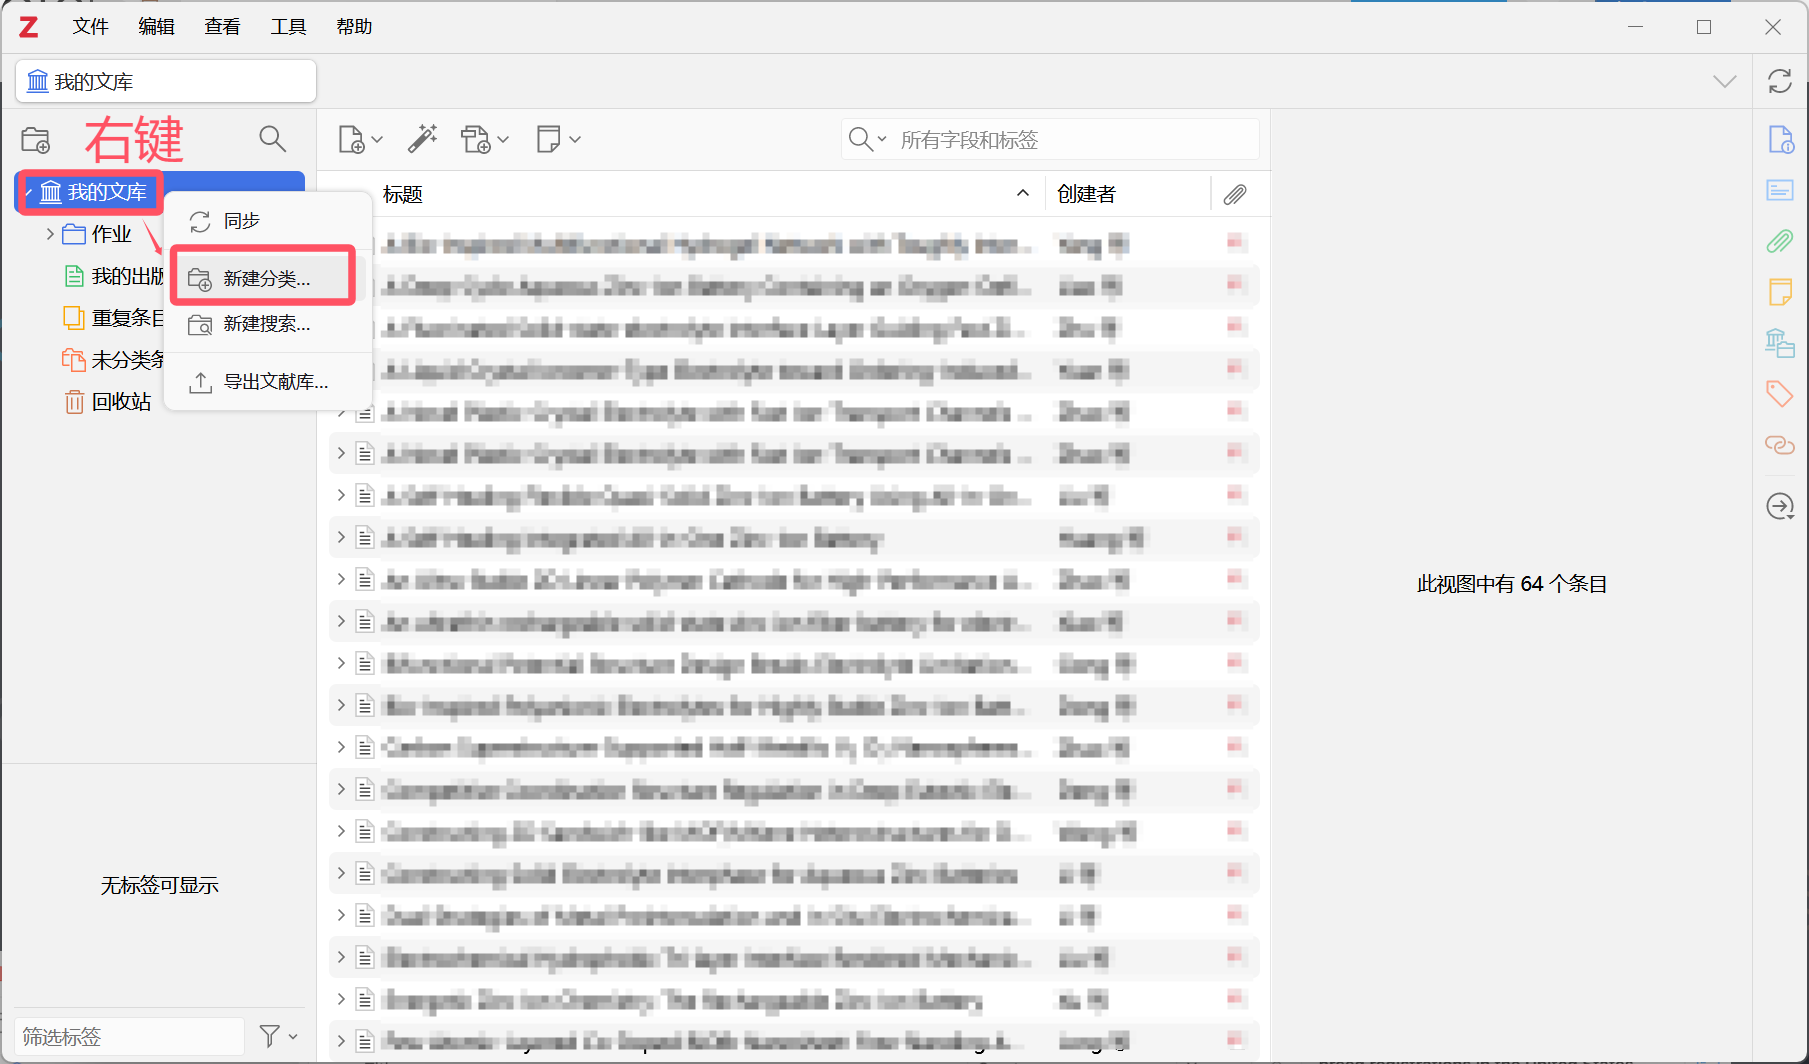
\includegraphics[width=0.8\textwidth]{Zotero打开.png}
        \caption{Zotero}
        \label{Zotero 1}
    \end{figure}
\end{lstlisting}
\end{minipage}
\end{center}

\newpage

\subsection{高阶命令}

\LaTeX{}可以实现很多你甚至想不到的功能。
随着学习的深入,你会认识到这是一个十分强大的工具。

高阶命令就不做介绍了,比如绘制表格、画图等等,有兴趣自行学习。

举个例子,\LaTeX{}中支持用TikZ绘图,精准但很麻烦。
在此不做介绍,只给出本文中例子,即学习曲线对比图:
\begin{center}
\begin{minipage}{0.8\textwidth}
    \hspace{1em}
\begin{lstlisting}[language={[LaTeX]TeX}]
    \begin{figure}[!h]
        \centering
        \captionsetup{font={small, bf}, margin=60pt}
        \begin{tikzpicture}[
            >=stealth,clip=true,scale=0.75
        ]
            \draw[->, thick] (0,0) -- (6.5,0) node[right] {\small 学习成本};
            \draw[->, thick] (0,0) -- (0,6.7) node[left, rotate=270, xshift=2.7cm, yshift=-0.4cm] {\small 熟练程度/效率};
        
            \draw[blue, thick, domain=0:6.5] 
                plot(\x, {(exp(0.4*\x) -1)*0.5}) node[right] {\LaTeX};
            \draw[red, thick, domain=0:6.5] 
                plot(\x, {(ln(\x +1))*2}) node[right] {Word};
        
            \draw[fill=white] (1.5,5) rectangle (5.2,6.2);
            \draw[blue,thick] (1.7,5.8) -- (2.3,5.8) node[right,black] {\small\LaTeX 曲线};
            \draw[red,thick] (1.7,5.3) -- (2.3,5.3) node[right,black] {\small Word曲线};
        
        \end{tikzpicture} 
        \caption{学习曲线对比图} 
    \end{figure} 
\end{lstlisting}
\end{minipage}
\end{center}

\newpage

\subsection{导入参考文献}

\newcommand{\BibTeX}{\textsc{B\kern-0.1emi\kern-0.017emb}\kern-0.15em\TeX}
\LaTeX{}可以方便地用\BibTeX{}管理参考文献,同样以Zotero为例,右键导出,选择\BibTeX{}(不选导出笔记),
导出到工作文件夹(这里是“演示”)为references.bib:

\begin{figure}[h]
    \centering
    \captionsetup{font={small, bf}, margin=60pt}
    \begin{subfigure}[c]{0.24\textwidth}
      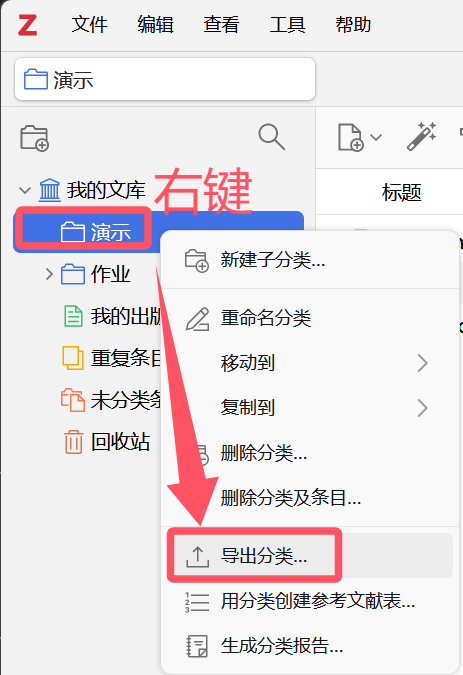
\includegraphics[width=\textwidth]{bib1.png}
      \label{bib 1-1}
    \end{subfigure}
    \hfill
    \begin{subfigure}[c]{0.20\textwidth}
      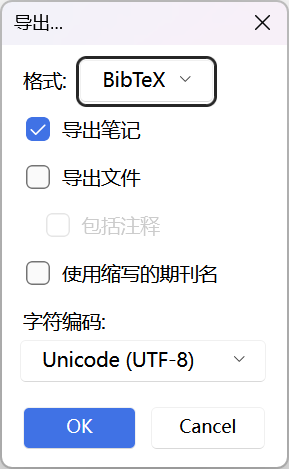
\includegraphics[width=\textwidth]{bib2.png}
      \label{bib 1-2}
    \end{subfigure}
    \hfill
    \begin{subfigure}[c]{0.47\textwidth}
      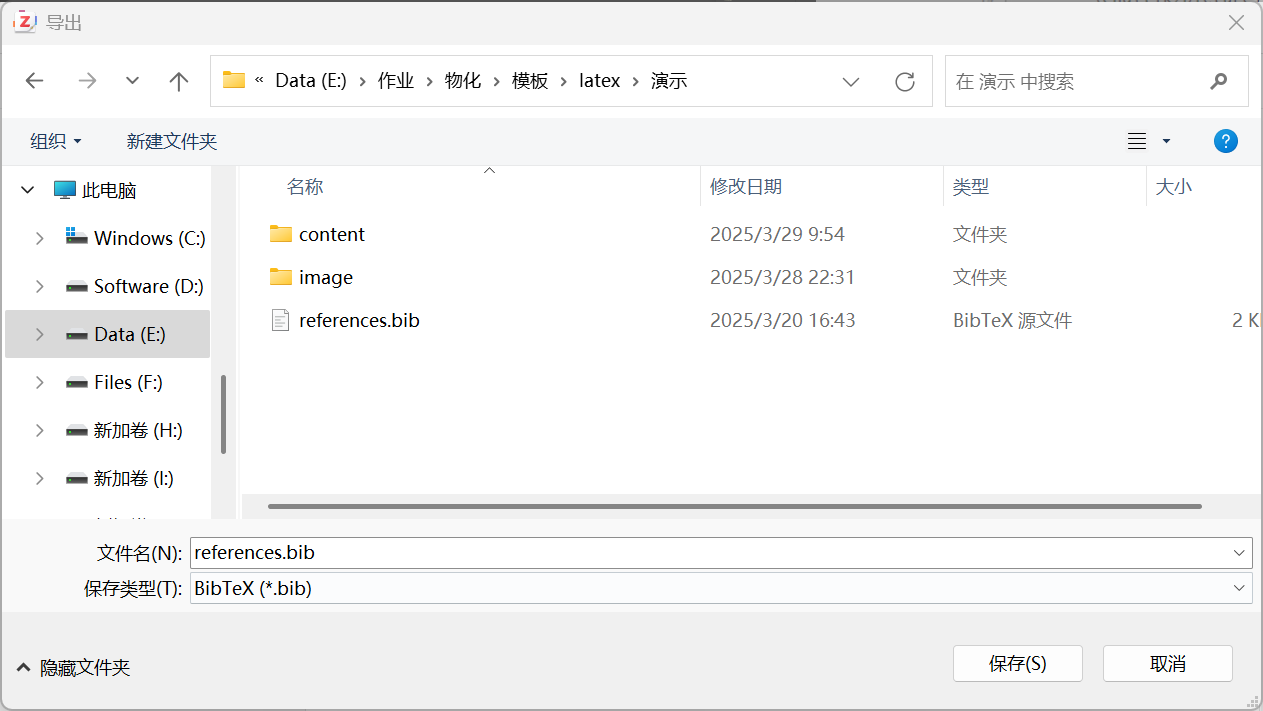
\includegraphics[width=\textwidth]{bib3.png}
      \label{bib 1-3}
    \end{subfigure}
    \caption{导出为references.bib}
    \label{bib 1}
\end{figure}

打开references.bib备用(可在VS Code里直接打开),
这次导入的第三个参考文献是从网页上直接导入的,里面有可以预先在Zotero文献信息中删除“其他”内容,
也可在references.bib文件手动删除“note=”这一行,以下即为\BibTeX{}文件(每个文献只展示前三行):

\begin{center}
\begin{minipage}{0.8\textwidth}
    \hspace{1em}
\begin{lstlisting}[language={[LaTeX]TeX}]
@article{zhao_novel_2023,
	title = {A {Novel} {Plastic}‐{Crystal} ...
	volume = {13},
    ...

@article{zhou_simultaneous_2024,
	title = {Simultaneous {Inhibition}...
	volume = {63},
    ...

@article{montes-tolentino_control_2025,
	title = {Control of {Interlocking} ...
	volume = {64},
    ...

\end{lstlisting}
\end{minipage}
\end{center}

\newcommand{\BibLaTeX}{\textsc{B\kern-0.1emi\kern-0.017emb}\kern-0.15em\LaTeX}
使用一些宏包能有其它的引用样式,也能调整是否显示链接或DOI等信息。这里不再赘述,可自行探索。

还可以使用更高级的\BibLaTeX{},可以通过参数直接调整想要显示的作者数量。这里不作演示,可自行学习。

引用时,bib文件中每条文献的第一行花括号右边就是标签,可以自行修改,但不建议(这里方便演示已分别改为a、b、c)。
按如下使用\backslash cite命令:
\begin{center}
\begin{minipage}{0.8\textwidth}
    \hspace{1em}
\begin{lstlisting}[language={[LaTeX]TeX}]
    示例文本:这里引用文献\cite{b},这里引用多个文献\cite{a, b, c}。
\end{lstlisting}
\end{minipage}
\end{center}
效果:

示例文本:这里引用文献\cite{b},这里引用多个文献\cite{a, b, c}。

同时,文档末尾会按照引用顺序生成引用文献列表,比如我这里的顺序是bac。
bib文献中有,但正文中未引用的文献也会排列在后面。

效果见本文档结尾。

还有更高级的交叉引用,如\backslash citet、\backslash citep、\backslash ref等等,
可以有多种引用,也可以引用文中的图片、表格等。这里不作介绍,可自行学习。

\subsection{编译}

编写好文档之后,如果你按照开头介绍的知乎文章正确配置的话,
就可以开始编译了,VS Code左边栏选择\TeX{},点击“构建\LaTeX{}项目”左边展开。

如果文章没有参考文献,点击\XeLaTeX{}开始编译,此时会报错,然后再点击编译一次,让章节信息进入目录即可。

如果文章有参考文献,点击\XeLaTeX{}->\BibTeX{}->\XeLaTeX{}*2,
一共会编译四次,第一次预编译,第二次导入参考文献,三四次则是执行两次正式编译,使目录也正常显示。